%        File: hw1.tex
%     Created: Sat Apr 06 10:00 AM 2013 P
% Last Change: Sat Apr 06 10:00 AM 2013 P
%
\documentclass[11pt]{article}

\usepackage{amsmath, amssymb, amsthm, cite, graphicx, float, mathrsfs, commath, dsfont, bbm, bm, setspace}
\usepackage[mathscr]{eucal}
\usepackage[sc]{mathpazo}
\linespread{1.05}
%\usepackage{setspace}
%\onehalfspacing
\usepackage[margin=1in, top=.8in, left=.8in]{geometry}
\usepackage{color}

% new commands
\DeclareMathOperator*{\argmin}{arg\,min}
\DeclareMathOperator{\sgn}{sgn}
\newcommand{\E}{\mathrm{E}}
\newcommand{\Var}{\mathrm{Var}}
\newcommand{\Cov}{\mathrm{Cov}}
\newcommand{\Cor}{\mathrm{Cor}}
\newcommand{\id}{\operatorname{id}}
\newcommand{\diag}{\operatorname{diag}}
\newcommand{\Id}{\operatorname{Id}}
\newcommand{\tr}{\operatorname{tr}}
\newcommand{\Q}{\mathbb{Q}}
\newcommand{\C}{\mathbb{C}}
\newcommand{\R}{\mathbb{R}}
\newcommand{\Z}{\mathbb{Z}}
\newcommand{\F}{\mathbb{F}}
\newcommand{\N}{\mathbb{N}}

\newcommand{\indep}{\rotatebox[origin=c]{90}{$\models$}}

% 524 commands
%\newcommand{\norm}[1]{\| #1 \|}
\DeclareMathOperator{\spn}{span}
%\newcommand{\spn}{\operatorname{span}}
\newcommand{\onenorm}[1]{\| #1 \|_{L^1(\mathbb R^d)}}
\newcommand{\twonorm}[1]{\| #1 \|_{L^2(\mathbb R^d)}}

% 534 commands
\renewcommand{\Re}{\text{Re\,}}
\renewcommand{\Im}{\text{Im\,}}

\begin{document}
\pagestyle{empty}
\hfill Abraham Engle

\hfill Stat 571

\hfill \today
\begin{enumerate}
    %1
	\item We are interested in the simple linear regression of an outcome $Y$ on one covariate $X$ and an intercept, allowing for clustering.
		\begin{enumerate}
			\item Using the notation from class, the vector of outcomes and the matrix of covariates in the $i$th cluster, $i=1,2,\dotsc,n$ is
			\[
				\bm{Y}_i = \begin{pmatrix}
				Y_{i1} \\ Y_{i2} \\ \vdots \\ Y_{in_i}
				\end{pmatrix}\quad\quad \bm{X}_i = \begin{pmatrix}
				1 & x_{i1} \\ 1 & x_{i2} \\ \vdots & \vdots \\
				1 & x_{in_i}
				\end{pmatrix}
			\]
			In the simple linear regression case, our function of the mean $g$ is just the identity, and the working correlation matrix is the identity matrix. In this case, the estimating equation takes the form
			\[
				\sum_{i=1}^n \bm{X}_i^T(\bm{Y}_i-\bm{X}_i\beta) = \bm{0}_2,
			\]
			where $\beta = (\beta_0,\beta_1)^T$ are the parameters of interest. Substituting the rules for $\bm{X}_i$ and $\bm{Y}_i$, we have
			\[
				\sum_{i=1}^n \begin{pmatrix}
				1 & 1 & \cdots & 1 \\
				x_{i1} & x_{i2} & \cdots & x_{in_i}
				\end{pmatrix}\begin{pmatrix}
				Y_{i1} - \beta_0 - \beta_1 x_{i1} \\ Y_{i2} - \beta_0 - \beta_1x_{i2} \\ \vdots \\ Y_{in_i} - \beta_0 - \beta_1x_{in_i}
				\end{pmatrix} = \bm{0}_2.
			\]
			This gives two equations:
			\begin{align*}
				\sum_{i=1}^n \sum_{j=1}^{n_i}(Y_{ij} - \beta_0 - \beta_1 x_{ij}) &= 0\\
				\sum_{i=1}^n \sum_{j=1}^{n_i}x_{ij}(Y_{ij} - \beta_0 - \beta_1 x_{ij}) &= 0.
			\end{align*}
			Using linearity and the fact that $\beta_0$ and $\beta_1$ are constant with respect to the summation variables $i,j$, we have
			\begin{align*}
				\beta_0\sum_{i=1}^n n_i + \beta_1 \sum_{i=1}^n \sum_{j=1}^{n_i} x_{ij} &= \sum_{i=1}^n \sum_{j=1}^{n_i} Y_{ij} \\
				\beta_0\sum_{i=1}^n\sum_{j=1}^{n_i} x_{ij} + \beta_1 \sum_{i=1}^n\sum_{j=1}^{n_i} x_{ij}^2 &= \sum_{i=1}^n \sum_{j=1}^{n_i} x_{ij}Y_{ij}.
			\end{align*}
			These are two linear equations in unknowns $\beta_0,\beta_1$, so we can write this in matrix form as
			\[
				\begin{pmatrix}
					n_\cdot & x_{\cdot\cdot} \\ x_{\cdot\cdot} &\sum_{i,j}x_{ij}^2
				\end{pmatrix}\begin{pmatrix}
				\beta_0 \\ \beta_1
				\end{pmatrix} = \begin{pmatrix}
				Y_{\cdot\cdot} \\ \sum_{i,j} x_{ij}Y_{ij},
				\end{pmatrix}
			\]
			where a dot in the subscript means that index has been summed over, for example $n_\cdot = \sum_{i=1}^n n_i$. Inverting the $2\times 2$ coefficient matrix, the formula for $\widehat{\beta}_1$ is
			\[
				\widehat{\beta}_1 = \frac{n_\cdot \sum_{i,j} x_{ij}Y_{ij} - x_{\cdot\cdot}Y_{\cdot\cdot}}{n_\cdot\sum_{i,j}x_{ij}^2 - (x_{\cdot\cdot})^2},
			\]
			and all that's left is to show that this is quantity is equal to
			\[
				\frac{1}{n_\cdot}\sum_{i,j} V^{-1}(x_{ij}-\bar{x})Y_{ij} = \frac{\sum_{i,j}(x_{ij}-\frac{x_{\cdot\cdot}}{n_\cdot})Y_{ij}}{\sum_{i,j} (x_{ij} - \frac{x_{\cdot\cdot}}{n_\cdot})^2},
			\]
			with $V = \frac{1}{n_\cdot}\sum_{i,j}(x_{ij}-\bar{x})^2$. Dividing both numerator and denominator of my expression by $n_\cdot$, we get
			\[
				\widehat{\beta}_1 = \frac{\sum_{i,j} x_{ij}Y_{ij} - \frac{x_{\cdot\cdot}Y_{\cdot\cdot}}{n_\cdot}}{\sum_{i,j}x_{ij}^2 - \frac{(x_{\cdot\cdot})^2}{n_\cdot}},
			\]
			and the numerators of both expressions match since we can write out the sum $Y_{\cdot\cdot}$ and the term in front is constant:
			\[
				\sum_{i,j} x_{ij}Y_{ij} - \frac{x_{\cdot\cdot}Y_{\cdot\cdot}}{n_\cdot} = \sum_{i,j} (x_{ij} - \frac{x_{\cdot\cdot}}{n_\cdot})Y_{ij}
			\]
			Similarly, the denominators match since if we expand the square in the denominator of the expression on the midterm, we have
			\[
				\sum_{i,j} (x_{ij} - \frac{x_{\cdot\cdot}}{n_\cdot})^2 = (\sum_{i,j} x_{ij}^2) - 2 \frac{(x_{\cdot\cdot})^2}{n_\cdot} + n_\cdot\frac{x_{\cdot\cdot}^2}{(n_\cdot)^2} = \sum_{i,j} x_{ij}^2 - \frac{(x_{\cdot\cdot})^2}{n_\cdot}
			\]
			as required.
			\item In terms of the expression on the midterm, we have
			\begin{align*}
				\Var(\widehat{\beta}_1) &= \left(\frac{1}{n_\cdot V}\right)^2\Var\left(\sum_{i,j} (x_{ij}-\bar{x})Y_{ij}\right) \\
				&= \left(\frac{1}{n_\cdot V}\right)^2\Cov\left(\sum_{i,j} (x_{ij}-\bar{x})Y_{ij},\sum_{k,l}(x_{kl}-\bar{x})Y_{kl}\right) \\
				&= \left(\frac{1}{n_\cdot V}\right)^2\sum_{i,j,k,l} (x_{ij}-\bar{x})(x_{kl}-\bar{x})\Cov\left(Y_{ij},Y_{kl}\right) \\
				&=\left(\frac{1}{n_\cdot V}\right)^2\sum_{i,j,l} (x_{ij}-\bar{x})(x_{il}-\bar{x})\Cov\left(Y_{ij},Y_{il}\right),
			\end{align*}
			where the first equality is due to the fact that $n_\cdot$ and $V$ are non-random and constants in the summations like we noted in (a). The second equality is the definition of the variance of a random variable. The third equality is from bilinearity of covariance and the observation that terms $(x_{ij}-\bar{x})$ and $(x_{kl}-\bar{x})$ are non-random. The last equality follows from the fact that we assume $k\neq i \Rightarrow \Cov(Y_{ij},Y_{kl}) = 0 $ for all $j,l$. \\ \\If the terms were not clustered, we would further assume $j\neq l\Rightarrow \Cov(Y_{ij},Y_{il})=0$ for all $i=1,2,\dotsc,n$, which would enable us to write the variance of the sum in the first line as the sum of variances, so
			\[
				\Var(\widehat{\beta}_1) = \left(\frac{1}{n_\cdot V}\right)^2\sum_{i,j} (x_{ij}-\bar{x})^2\Var\left(Y_{ij}\right)
			\]
			
			\item I obtain estimates of the terms $\Cov(Y_{ij},Y_{il})$ for $i=1,2,\dotsc,n$ and $j,l=1,2,\dotsc,n_i$, from the theoretical definition:
			 \[
			 	\Cov(Y_{ij},Y_{il}) = E[(Y_{ij} - E[Y_{ij}])(Y_{il} - E[Y_{il}]),
			 \]
			 so my estimate is
			 \[
			 	\widehat{\Cov}(Y_{ij},Y_{il}) = (Y_{ij}-\widehat{\beta}_0 - \widehat{\beta}_1x_{ij})(Y_{il}-\widehat{\beta}_0 - \widehat{\beta}_1x_{il})
			 \]
			 Since there is only one variance, the meat and bread must necessarily be real numbers. This is because we're inverting $A$, so it has to be square and the dimension must be one by comparing with the dimension of the estimate. If $\widehat{A}$ is a real number, then it follows the meat $B$ must also be a real number. Our estimate takes the form
			 \begin{align*}
			 	\widehat{\Var}(\widehat{\beta}_1) &= \left(\frac{1}{n_\cdot V}\right)^2\sum_{i=1}^n \sum_{j=1}^{n_i}\sum_{l=1}^{n_i} (x_{ij}-\bar{x})(Y_{ij}-\widehat{\beta}_0 - \widehat{\beta}_1x_{ij})(Y_{il}-\widehat{\beta}_0 - \widehat{\beta}_1x_{il})(x_{il}-\bar{x}) \\
			 	&= \left(\frac{1}{n_\cdot V}\right)^2\sum_{i=1}^n \sum_{j=1}^{n_i}(x_{ij}-\bar{x})(Y_{ij}-\widehat{\beta}_0 - \widehat{\beta}_1x_{ij})\sum_{l=1}^{n_i}(x_{il}-\bar{x})(Y_{il}-\widehat{\beta}_0 - \widehat{\beta}_1x_{il}) \\
			 	&=  \left(\frac{1}{n_\cdot V}\right)^2\sum_{i=1}^n \left(\sum_{j=1}^{n_i}(x_{ij}-\bar{x})(Y_{ij}-\widehat{\beta}_0 - \widehat{\beta}_1x_{ij})\right)^2 \\
			 	&= \frac{\sum_{i=1}^n \left(\sum_{j=1}^{n_i}(x_{ij}-\bar{x})(Y_{ij}-\widehat{\beta}_0 - \widehat{\beta}_1x_{ij})\right)^2}{(n_\cdot V)^2} \\
			 	&= \frac{\sum_{i=1}^n \left(\sum_{j=1}^{n_i}(x_{ij}-\bar{x})(Y_{ij}-\widehat{\beta}_0 - \widehat{\beta}_1x_{ij})\right)^2}{(\sum_{i=1}^n\sum_{j=1}^{n_i}(x_{ij}-\bar{x})^2)^2} \\
			 	&=: \frac{\widehat{B}}{(\widehat{A})^2}
			 \end{align*}
			To verify these estimates agree with what's theoretically given 2.23 in a non-algebraic way, I ran a GEE on the dental data from class using an independence working correlation assumption and running a simple linear regression of the distance against age.
		\end{enumerate}
	
	%2
	\item Continuing the hypothetical situation with $n$ test scores in English and math, I suppose $Y_{i1}$ is the math score and $Y_{i2}$ is the English score. Let $U_i$ be an indicator of whether the $i$th student had a particular English professor and let $X_i$ be an indicator of whether the $i$th student had a particular math professor. We wish to implement a linear regression of $Y_{i1}$ on $X_i$ adjusting for $Z_i$ and $Y_{i2}$ on $U_i$ adjusting for $Z_i$, where $Z_i$ is some other covariate of interest, for example the age of the $i$th student. The mean model I fit is
		\[
			E[Y_{ij}|Z_i,X_i,U_i] = \beta_0 + \beta_1\mathrm{English}_i + \beta_2Z_i + \beta_3[\bm{1}_{j=1}X_i] + \beta_4[\bm{1}_{j=2}U_i] + \beta_5Z_i[\bm{1}_{j=1}X_i] + \beta_6Z_i[\bm{1}_{j=2}U_i]
		\]
		or in components, the mean model is
		\begin{align*}
			E[Y_{i1}|Z_i,X_i,U_i] &= \beta_0 + \beta_2 Z_i + \beta_3 X_i + \beta_5 Z_iX_i\\
			E[Y_{i2}|Z_i,X_i,U_i] &= \beta_0 + \beta_1 + \beta_2 Z_i + \beta_4 U_i + \beta_6 Z_iU_i
		\end{align*}
	Since we are adjusting for $Z_i$ in both mean models and since they both share the parameter $\beta_1$, I would make sure that my outcomes (in this case, test scores) are on the same scale before fitting the model with GEE. I would also implement my $Z_i$ age variable as something like we did in class: $Z_i = \mathrm{Age}_i-18$, which just helps with interpretation. My parameters are
	\begin{itemize}
		\item $\beta_0$: Mean test score in math at age 18 for those not having the particular math professor.
		\item $\beta_1$: Difference in mean test scores in math and English among students at age 18 not having either particular professor.
		\item $\beta_2$: Difference in mean math test score per additional year of age in students not having the math professor. OR Difference in mean English test score per additional year of age in students not having the particular English professor.
		\item $\beta_3$: Among eighteen year olds, the difference in math test score between students who had the particular math professor and those who did not.
		\item $\beta_4$: Among eighteen year olds, the difference in English test score between students who had the particular English professor and those who did not.
		\item $\beta_5$: Difference in the age effect, comparing those with the math professor and those without.
		\item $\beta_6$: Difference in the age effect, comparing those with the English professor and those without.
	\end{itemize}
	I am concerned with fitting a model with so many parameters, since we get in to overfitting depending on how many students we have. I would definitely make sure to look at my data set before proposing a relatively large model like this one. When running the GEE, I would work with an exchangeable correlation assumption, since I believe test scores between subjects do have some correlation, like the example in the instructions with parental help. 
	\\ \\I generated some data and fit a model like this to test whether the parameter estimates were close to what I generated. In particular, I chose $\bm{\beta} = (60,-20,2,10,-10,3,-1)$ and generated 
	\begin{align*}
		Y_{i1}&\sim_{ind} N(\beta_0 + \beta_2 Z_i + \beta_3 X_i + \beta_5 Z_iX_i + W_i,1) \\
		Y_{i2}&\sim_{ind} N(\beta_0 + \beta_1 + \beta_2 Z_i + \beta_4 U_i + \beta_6 Z_iU_i + W_i,1),
	\end{align*}
	where the normality adds noise and I add $W_i$ to represent some external factor like parental help, that my GEE attempts to account for with the working correlation. I generated 20 students of differing ages between age 13 to 23, randomly divided half of them into the math class, separately divided another random half of them into an English class, and separately chose another random half to have strong parental help ($W_i=5$). Having equal number of clusters with the given age, I repeated this 1000 times to have 20,000 students' test scores according to the model above. I ran GEE with exchangeable working correlation and found
	\begin{verbatim}
running glm to get initial regression estimate
(Intercept)         int           Z           X           U         Z:X         Z:U 
 62.5428840 -20.0289279   1.9983790   9.9173050 -10.0362579   2.9995071  -0.9982218 

Model:
 Link:                      Identity 
 Variance to Mean Relation: Gaussian 
 Correlation Structure:     Exchangeable 

Call:
gee(formula = value ~ int + Z + X + U + Z * X + Z * U, id = id, 
    data = data, corstr = "exchangeable")

Number of observations :  40000 

Maximum cluster size   :  2 


Coefficients:
(Intercept)         int           Z           X           U         Z:X         Z:U 
  62.519052  -19.992097    2.001091    9.965075  -10.062310    2.995918   -1.005674 

Estimated Scale Parameter:  7.242355
Number of Iterations:  2

Working Correlation[1:4,1:4]
          [,1]      [,2]
[1,] 1.0000000 0.8615856
[2,] 0.8615856 1.0000000
	\end{verbatim}
	We've misspecified the mean model, so our estimate for the $\beta_0$ is slightly off, but the others do look mostly correct. The initial regression estimate uses independence working correlation, and our estimates do not differ much from those. However, GEE with the exchangeable working correlation takes into account the correlation present in the data.
 	%3
	\item 
		\begin{enumerate}
			\item Suppose we know $\alpha$, the ARE, and the Power of the test based on the Wald statistic when the efficient covariance structure is used in the GEE analysis. Let 
			\[
				c = \frac{\Var(\widehat{\beta})_E}{\Var(\widehat{\beta})_I}
			\]
			denote the asymptotic relative efficiency of the inefficient compared to the efficient covariance structures, so that $\mathrm{SE}(\widehat{\beta})_I = \frac{\mathrm{SE}(\widehat{\beta})_E}{\sqrt{c}}$. We start with the formula for the power:
			\begin{align*}
				P_E &= 1 - \Phi\left(Z_{1-\alpha} - \frac{\beta}{\mathrm{SE}(\widehat{\beta})_E}\right),
			\end{align*}
			which, after rearranging, gives
			\[
				Z_{1-\alpha} - \Phi^{-1}(1-P_E) = \frac{\beta}{\mathrm{SE}(\widehat{\beta})_E},
			\]
			and we know all quantities on the left-hand side since we know $\alpha$, hence we can write
			\[
				\frac{\sqrt{c}\beta}{\mathrm{SE}(\widehat{\beta})_E} = \sqrt{c}\left(Z_{1-\alpha} - \Phi^{-1}(1-P_E)\right)
			\]
			entirely in terms of known quantities since we also know the number $c>0$. It follows that
			\[
				P_I = 1-\Phi\left(Z_{1-\alpha} - \frac{\sqrt{c}\beta}{\mathrm{SE}(\widehat{\beta})_E}\right) = 1 - \Phi\left(\left(1-\sqrt{c}\right)Z_{1-\alpha} + \Phi^{-1}(1-P_E)\right).
			\]
			\item Since the power is a number in the interval $[0,1]$, I plot the power of the efficient estimate on the horizontal axis against values of the inefficient estimate on the veritcal axis for $\alpha = 0.05$ and $c:=ARE = 0.1,0.3,0.5,0.7,$ and $0.9$. The figure is
			\begin{figure}[H]
				\centering
				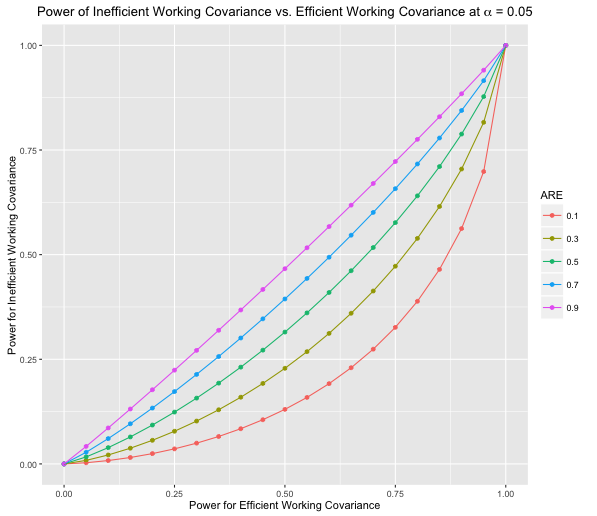
\includegraphics[scale=0.5]{Rplotp31}
			\end{figure}
		The most obvious feature for all choices of $ARE$ is that the power in the inefficient case is strictly smaller than the power reported in the efficient case (except at the endpoints). For ARE's close to one, the curve looks more and more like the identity line $y=x$, but as the ARE tends to zero, it looks like we bend farther away from the identity line for all values of the power except for zero and one.
		\item Setting $\alpha = 10^{-6}$, the figure is
			\begin{figure}[H]
				\centering
				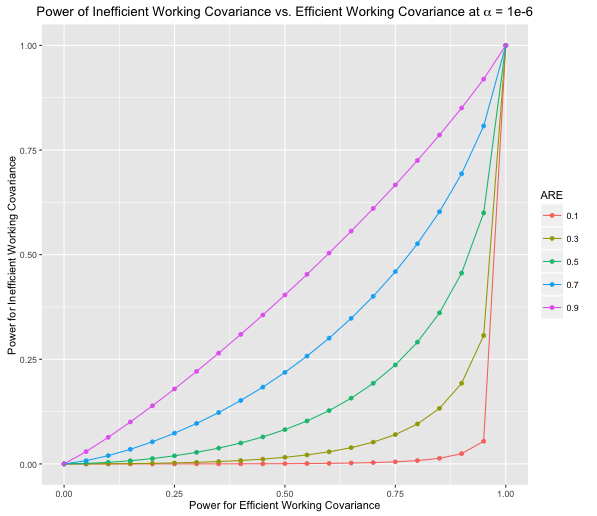
\includegraphics[scale=0.5]{Rplotp32}
			\end{figure}
		The same general features that we noted in (a) reappear here, the main difference between the two figures to me is how exaggerated the difference in powers becomes as the ARE lowers. Our choice of $ARE=0.1$ gives powers from the inefficient assumption very close to zero regardless of the power of the efficient estimate, but still giving equal powers at 0 and 1.
		\end{enumerate}
	%4
	\item
		\begin{enumerate}
		\item The number of clusters is an an integer multiple of 20, so we can have equal numbers of clusters with $b_i = \sigma\Phi^{-1}((1-0.5/20)),\sigma\Phi^{-1}((2-0.5)/20),\dotsc,\sigma\Phi^{-1}((20-0.5)/20)$. I took $n = 20\times10^3$ clusters and generated data according to the model in the instructions. I computed two GEE logistic regressions of $Y$ on $X$ and $Z$ with independent and exchangeable working covariance assumptions. I obtained the 3 robust standard errors from the outputs of both regressions and formed 3 ratios from the two regressions, with the robust standard errors from the independence model in the denominator. I did this for values of $\sigma\in\{0.5,1,\dotsc,3\}$ and fixing $\bm{\beta} = (-2.5,1,1)$.
%			\item The efficient estimate is from the independence working correlation. The mean model is misspecified, marginal mean, because logistic regression.. don't see as much as from linear regression.
				\begin{table}[H]
				\centering
				\begin{tabular}{|r||r|r|r|}
				  \hline
				 $\sigma$ & $\beta_0$ & $\beta_1$ & $\beta_2$ \\ 
				  \hline
				0.5 & 1.00 & 1.00 & 1.00 \\ 
				  1 & 1.00 & 1.00 & 1.00 \\ 
				 1.5 & 1.00 & 1.00 & 1.00 \\ 
				  2 & 1.00 & 1.00 & 1.00 \\ 
				  2.5 & 1.00 & 1.00 & 1.00 \\ 
				  3 & 0.99 & 1.00 & 0.99 \\ 
				   \hline
				\end{tabular}
				\caption{ARE with no Missing Data}
				\end{table}
			
			\item When we censor the last 3, the ARE is no longer nearly 1 for all choices of $\sigma$. We have smaller ARE across all parameters for larger values of $\sigma$. 
%				When there is correlation (like there is right now, the $Y_{ij}$s are correlated from  the data generating mechanism), we place more weight in computing estimates on the full observations.
				\begin{table}[H]
				\centering
				\begin{tabular}{|r||r|r|r|}
 				 \hline
				 $\sigma$ & $\beta_0$ & $\beta_1$ & $\beta_2$ \\ 
 				 \hline
 				 \hline
				0.5& 1.00 & 1.00 & 1.00 \\ 
				  1 & 1.00 & 0.99 & 0.99 \\ 
				  1.5 & 0.99 & 0.96 & 0.98 \\ 
				  2 & 0.98 & 0.92 & 0.97 \\ 
				  2.5 & 0.97 & 0.87 & 0.97 \\ 
				  3 & 0.97 & 0.84 & 0.96 \\ 
				   \hline
			\end{tabular}
			\caption{ARE with Half Clusters Missing Latter 3 Observations}
			\end{table}
		\end{enumerate}
	
	%5
	\item 
	{\setstretch{2.0}
	The paper proposes a new method of modeling longitudinal data in a way that mimics and extends what happens in generalized linear models without heavy model-based assumptions. The authors discuss some attractive statistical properties of the estimates they propose like consistency and asymptotic normality and conclude with discussing efficiency and robustness.
	\\ \\ The authors start out introducing notation that we learned in the second week of the course on slide 2.4 for clustering data, where they mention that typically clustering in data occurs whenever we have repeated measurements on an individuals $i=1,2,\dotsc,n$ at discrete times $t=1,2,\dotsc,n_i$. In the case of a single observation, $n_i=1$ for each individual, the methods and theory from 570 can be applied to the data, which allowed lots of models under the exponential family for the outcome based on whatever covariates were of interest. The authors go on to mention existing work in the case when $n_i>1$ and the outcome is Gaussian or binary, but that some of the difficulty in generalizing thesee model-based approaches was due to the difficulties in dealing with joint densities from arbitrary random vectors. 
	\\ \\ Sections 2 and 3 present the equations that need to be solved to obtain estimates $\widehat{\bm{\beta}}$. In section 2, the authors assume independence of outcomes within a cluster and use the score equations that arise from assuming a likelihood-based approach to motivate the full form of the GEE on slide 2.42 or equation (6) in the paper. After introducing the estimating equations in the second section, they give a theorem about consistency and asymptotic normality for the estimate $\widehat{\bm{\beta}}$ under ``mild regularity conditions" and present the limiting variance--and a consistent estimate thereof--in the sandwich form that we've seen throughout the year. Section 3 begins by addressing the efficiency loss the estimates in the previous section possess whenever within-cluster correlation is large. They go on to define the class of working correlation matrices we've seen and define the full set of GEEs. After presenting the equations, a theorem similar to that in section 2 is presented: if we have mild regularity conditions, consistent estimators of the scale and correlation parameters, and a boundedness condition on the derivative $\partial \widehat{\alpha}/\partial \phi$, the estimate $\widehat{\bm{\beta}}$ is again consistent and asymptotically normal with a slightly generalized limiting sandwich variance. 
	\\ \\
	Afterwards, the authors propose an algorithm to find $\widehat{\bm{\beta}}$ based on cycling between a Newton step and updating estimates of the parameters $\widehat{\alpha}$ and $\widehat{\phi}$. The end of section 3 and most of section 4 gives details on how the algorithm defines the estimators of the correlation and scale parameters in terms of Pearson residuals for different choices of working correlation matrices.
	\\ \\ Section 5 discusses asymptotic relative efficiency using the examples we've seen in class. When there is small correlation, there's not much difference between choices of working correlation; however, when outcomes are strongly correlated, we gain a lot of efficiency choosing the correct working correlation. They also mention a situation similar to problem 3(b) whenever we have unequal cluster sizes and correlation in the form of exchangeable outcomes. When cluster sizes are equal, there is no misweighting due to the inefficient estimate, but whenever cluster sizes are unequal, the incorrect weighting can lead to serious loss in efficiency
	\\ \\ At the very end of the paper, the authors summarize the properties of their proposed model: they treat different clusters as independent, avoid specifying joint distributions, and ``treat covariance structure... as a nuisance". They conclude with a discussion of robustness to misspecification of the mean model and working covariance, that we've seen summarized on slide 2.49.   \par}
\end{enumerate}
\newpage
R Code
\begin{verbatim}
	library(gee)
library(geeM)
library(ggplot2)
library(reshape2)
library(xtable)
########################
#######Problem 1########
########################
data(Orthodont, package="nlme")
d4 <- Orthodont # using shorter names
d4$id <- d4$Subject
d4$male <- d4$Sex=="Male"
glm1 <- glm(distance~I(age-8)*male, data=d4)
glm2 <- glm(distance~age, data=d4)
gee1 <- geem(distance~age, id=id, data=d4, corstr="independence")
X = model.matrix(glm2)
A = sum((X[,2]-mean(X[,2]))^2)
B = 0
for(i in seq(1,length(d4$distance),by=4))
{
  B = B + sum((X[i:(i+3),2]-11)*(d4$distance[i:(i+3)]-X[i:(i+3),]%*%gee1$beta))^2
}

B/A^2

bhat <- sum((X[,2]-mean(X[,2]))*d4$distance)/A
#agrees with gee1

########################
#######Problem 2########
########################
set.seed(200)
n = 20 #20 chirrens
beta0 = 60
beta1 = 40 #english is harder
beta2 = 2 #age, Z
beta3 = 10 #math, X
beta4 = -10 #english, U
beta5 = 3
beta6 = -1
i = 1
data = data.frame()
repeat
{
  english = sample(1:n,size=(n/2),replace=F)
  math = sample(1:n,size=(n/2),replace=F)
  Z = sample(-5:5,size=n,replace=T)
  y1 = rep(beta0,n)
  y2 = rep(beta1,n)
  y1[math] = y1[math] + beta3 + Z[math]*beta5
  y2[english] = y2[english] + beta4 + Z[english]*beta6
  W = rep(0,n) #parental help
  help = sample(1:n, size=(n/2),replace=F)
  W[help] = 5 #no help
  y1 = y1 + beta2*Z +  rnorm(n,0,1) + W
  y2 = y2 + beta2*Z + rnorm(n,0,1) + W
  mathind = rep(0,n)
  mathind[math] = 1
  engind = rep(0,n)
  engind[english] = 1
  
  tempdata = data.frame(cbind(y1,y2)) #write y2 as percentage points
  start = 20*(i-1) + 1
  tempdata$id = factor(start:(start+19))
  sort = melt(tempdata,id.var="id")
  sort = sort[order(sort$id),]
  sort$Z = rep(Z,each=2)
  sort$X = rep(mathind,each=2)
  sort$U = rep(engind,each=2)
  data = rbind(data,sort)
  if(i >= 1000)
  {
    break
  }
  i = i + 1
}

data$U[seq(1,dim(data)[1],by=2)]=0 #indicator turn odd off
data$X[seq(2,dim(data)[1],by=2)]=0
data$int = rep(1,dim(data)[1])
data$int[seq(1,dim(data)[1],by=2)]=0 #fit separate intercepts
gee(value~int+Z+X+U+Z*X+Z*U,id=id, data=data, corstr="exchangeable")

########################
#######Problem 3########
########################
PI <- function(alpha,c,PE)
{
  return(
    1 - pnorm(
      (1-sqrt(c))*qnorm(1-alpha) + qnorm(1-PE)
              )
    )
}


q3 = matrix(0,nrow=105,ncol=2)
q3[,1] = rep(seq(0,1,0.05),5)
cs = c(0.1,0.3,0.5,0.7,0.9)
inds = (0:4)*21 + 1
j = 1
for(ind in inds)
{
  q3[ind:(ind+20),2] = PI(0.05,cs[j],seq(0,1,0.05))
  j = j + 1
}

df = data.frame(q3)
names(df) = c("PE", "PI")
df$ARE <- rep(as.factor(cs),each=21)
ggplot(df, aes(x=PE, y=PI,col=ARE)) + geom_point() + geom_line() + 
ggtitle(expression(paste("Power of Inefficient Working Covariance vs. Efficient Working Covariance at ", alpha, " = 0.05"))) +
  
xlab("Power for Efficient Working Covariance") + ylab("Power for Inefficient Working Covariance")

#now do it for a new alpha
j = 1
for(ind in inds)
{
  q3[ind:(ind+20),2] = PI(1e-6,cs[j],seq(0,1,0.05))
  j = j + 1
}

df = data.frame(q3)
names(df) = c("PE", "PI")
df$ARE <- rep(as.factor(cs),each=21)
ggplot(df, aes(x=PE, y=PI,col=ARE)) + geom_point() + geom_line() + 
ggtitle(expression(paste("Power of Inefficient Working Covariance vs. Efficient Working Covariance at ", alpha, " = 1e-6"))) +
xlab("Power for Efficient Working Covariance") + ylab("Power for Inefficient Working Covariance")


########################
#######Problem 4########
########################
expit <- function(x)
{
  return(
    exp(x)/(1+exp(x))
  )
}
#part (a)
set.seed(1)
ARE = matrix(0,nrow=6,ncol=3) #one row per sigma, one column per coefficient
m = 10^3
n = 20*m #clusters are integral multiples of 20.
ni = 6 #same for each clsuter
#clusters have same X covariate
x = (1:6-3)/3
sigmas = seq(0.5,3,0.5)
#sigmas = 0.5
beta0 = -2.5
beta1 = 1
beta2 = 1
beta = c(beta0,beta1,beta2)

X = rep(x,n)
for(j in 1:length(sigmas))
{
  b = sigmas[j]*rep(qnorm(ppoints(20)),each=(ni*m))
  #fixing b this way puts clusters with equal values of b_i next to one another

  ones = sample(1:n,size=(n/2),replace=F)
  z = c()
  for(i in 1:n)
  {
    if(i %in% ones)
    {
      z = append(z,rep(1,6))
    }
    else{
      z = append(z,rep(0,6))
    }
  }
  
  probs = expit(cbind(rep(1,(n*ni)), X, z)%*%beta + b)
  Y = rep(0,(n*ni))
  for(i in 1:(n*ni))
  {
    Y[i] = rbinom(1,1,probs[i])
  }
  id = rep(1:n,each=6) #cluster id
  dat = data.frame(cbind(Y,X,z,id,b)) #make the data frame
  #COMMENT OUT FOR part(a)
  missing = sample(1:n, size=(n/2), replace=F) #which clusters to omit
  where = 6*(missing-1) + 1
  dat = dat[-c(where + 3 , where + 4, where + 5),]
  #Comment above... dont reseed
  geeIND = geem(Y~X+z,data=dat, id=id, family=binomial(link="logit"), corstr="independence")
  geeEXCH = geem(Y~X+z,data=dat,id=id, family=binomial(link="logit"), corstr="exchangeable")
  ARE[j,]=summary(geeEXCH)$se.robust/summary(geeIND)$se.robust
}


xtable(ARE)

\end{verbatim}
\end{document}



